\subsection{Papers With Code (SOTA Platform)}
{{\footnotesize
\noindent Papers With Code (PWC) aggregates benchmark suites, tasks, and code across ML research:
12,423 benchmarks, 5,358 unique tasks, and 154,766 papers with code links. It tracks SOTA metrics and fosters reproducibility.


\begin{description}[labelwidth=4cm, labelsep=1em, leftmargin=4cm, itemsep=0.1em, parsep=0em]
  \item[date:] ongoing
  \item[version:] v1.0
  \item[last\_updated:] 2025-06
  \item[expired:] unknown
  \item[valid:] yes
  \item[valid\_date:] ongoing
  \item[url:] \href{https://paperswithcode.com/sota}{https://paperswithcode.com/sota}
  \item[doi:] unknown
  \item[domain:] General ML; All domains
  \item[focus:] Open platform tracking state-of-the-art results, benchmarks, and implementations across ML tasks and papers
  \item[keywords:]
    - leaderboard
    - benchmarking
    - reproducibility
    - open-source
  \item[licensing:] Apache License 2.0
  \item[task\_types:]
    - Multiple (Classification, Detection, NLP, etc.)
  \item[ai\_capability\_measured:]
    - Model performance across tasks (accuracy
    - F1
    - BLEU
    - etc.)
  \item[metrics:]
    - Task-specific (Accuracy, F1, BLEU, etc.)
  \item[models:]
    - All published models with code
  \item[ml\_motif:]
    - Multiple
  \item[type:] Platform
  \item[ml\_task:]
    - Multiple
  \item[solutions:] 0
  \item[notes:] Community-driven open platform; automatic data extraction and versioning.

  \item[contact.name:] Papers With Code Team
  \item[contact.email:] unknown
  \item[results.links.name:] ChatGPT LLM
  \item[fair.reproducible:] Yes
  \item[fair.benchmark\_ready:] Yes
  \item[id:] papers\_with\_code\_sota\_platform
  \item[Citations:] \cite{pmlr-v37-blum15}
\end{description}

{\bf Ratings:} ~ \\

\begin{tabular}{p{0.15\textwidth} p{0.07\textwidth} p{0.7\textwidth}}
\hline
Rating & Value & Reason \\
\hline
dataset & 3 & Relies on external datasets submitted by the community. While links are available, FAIR compliance
is not guaranteed or systematically enforced across all benchmarks.
 \\
documentation & 4 & Strong front-end documentation and metadata on benchmarks, tasks, and models; however, some benchmark-specific
instructions are sparse or dependent on external paper links.
 \\
metrics & 5 & Tracks state-of-the-art using task-specific metrics like Accuracy, F1, BLEU, etc., with consistent
aggregation and historical SOTA tracking.
 \\
reference\_solution & 3 & Provides links to implementations of many SOTA models, but no single unified reference baseline
is required or maintained per benchmark.
 \\
software & 5 & Actively maintained open-source platform (https://paperswithcode.com) under Apache 2.0 license;
includes automatic integration with GitHub, datasets, and models for reproducibility.
 \\
specification & 4 & Task and benchmark structures are well organized and standardized, but due to its broad coverage,
input/output formats vary significantly between tasks and are not always tightly controlled.
 \\
\hline
\end{tabular}

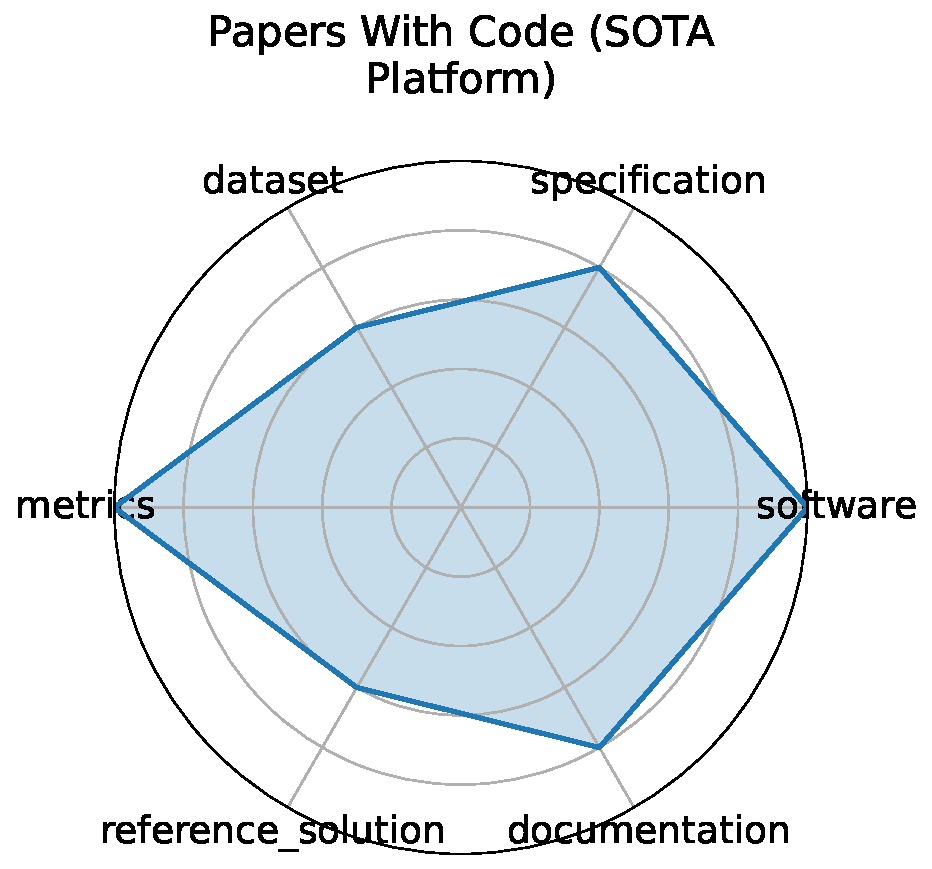
\includegraphics[width=0.2\textwidth]{papers_with_code_sota_platform_radar.pdf}
}}
\clearpage